%!TEX root = ./../thesis.tex

\chapter{State Centric Programming Model}
\label{c:state_centric}
Most state-of-the-art frameworks for distributed machine learning like Petuum \cite{Xing2015} and Parameter Server \cite{Li2014} are based on the parameter server concept introduced in the previous section.
The framework essentially provides a low level API\footnote{Application programming interface} for publishing and retrieving values similar to a distributed key-value store, where the key $i$ is for example the index of a weight vector $w$ stored on the server and the value is the weight $w_i$.
Implementing an algorithm that relies on a parameter server requires incorporating publishing and retrieval of parameters deeply into the algorithm definition.
This contrasts the general workflow of developing and testing an algorithm locally on a single machine and then transition to a distributed environment.
The parameter server paradigm also provides only a minor abstraction, leaving the developer with the task of distributing state, scheduling distributed computation, consistency management and managing cluster resources.
A developer should be able to focus on the key elements necessary for efficient parallel execution of distributed machine learning algorithms.
In this section these elements and the overall architecture of the framework is explained based on the example of iterative-convergent algorithms in general, though it is not limited to this particular group.
The result is a state centric programming model, treating state as a first class citizen that can be distributed and altered by local and remote transformation in parallel.
Depending on how state is distributed and the kind of transformation applied to it, the consistency management is then responsible for ensuring an efficient but correct execution of all algorithm steps.
Algorithm \ref{alg:general_ica} contains the generic definition of an iterative-convergent algorithm as it would be implemented by a developer.
The flow is very similar among members of the ICA\footnote{iterative-convergent-algorithm} family, except that $f_p$ and $\Delta(\ldots)$ are replaced by the corresponding preprocessing transformation respectively the optimization technique employed for iteratively approximating the optimal solution according to Section \ref{ss:optimization}.
\begin{algorithm}
\caption{Generic iterative-convergent algorithm definition}\label{alg:general_ica}
\begin{algorithmic}[1]{}
\ALGSTATE Data tensor $D \in \mathbb{R}^{n \times d}$, weight tensor $w \in \mathbb{R}^{m \times d}$
\INPUT algorithm specific hyperparameters $\theta$, if any
\INIT $t \gets 0$, $w^{(0)} \gets 0$
\State $D \gets f_{p}(D)$ \Comment{(A)}
\Repeat \Comment{(B)}
\State $t \gets t + 1$
\State $w^{(t)} \gets w^{(t-1)} + \Delta(w^{(t-1)}, \theta, D)$ \Comment{(C)}
\Until{termination criteria satisfied} \Comment{(D)}
\end{algorithmic}
\end{algorithm}
An algorithm expressed in this form can be executed as is on a single machine without modification but in order to distribute it among a cluster of machines the algorithm definition must be translated into a representation describing the logical sequence of transformations, the state that is used in each transformation and instructions for the consistency management so each transformation can be executed in a distributed environment without loosing its correctness.
This intermediate representation (logical plan) can then be combined with information about the cluster resources to obtain a physical plan, which can be used by the framework to actually schedule the distributed execution of the algorithm in a cluster.
The sequence of steps necessary to go from an algorithm definition to a distributed or physical plan is depicted in Figure \ref{fig:parallel_pipeline}, where a light arrow resembles an intermediate representation and a dark arrow depicts a transformation step between those representations.
At each step, the corresponding representation is enriched by additional information about the algorithm or cluster infrastructure.
\begin{figure}[ht]
\centering
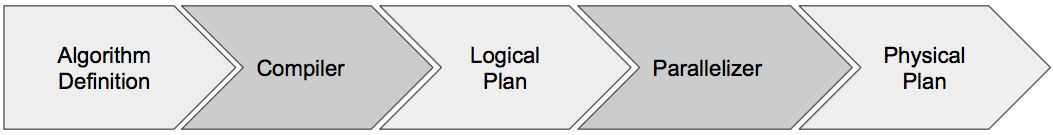
\includegraphics[width=0.9\textwidth]{img/algo_parallel_pipeline.png}
\caption{Algorithm parallelization pipeline}
\label{fig:parallel_pipeline}
\end{figure}
The following sections describe how the intermediate representations look like and what purpose they serve.

\section{Intermediate Representations}

\subsection{Logical Plan}
In the first step, a logical plan is derived from the algorithm definition, the compiler identifies the building blocks of the given algorithm such as control flow, transformations and state present in the algorithm as well as the dependencies among them.
The information used to derive the logical plan is solely based on the algorithm definition and does not take infrastructure related properties into account.
At first, the logical control flow is derived from the algorithm definition (\ref{alg:general_ica}) describing the training process of an ICA such as linear regression, support-vector machine or logistic regression, as can be seen in Figure \ref{fig:general_pipeline}.
\begin{figure}[ht]
\centering
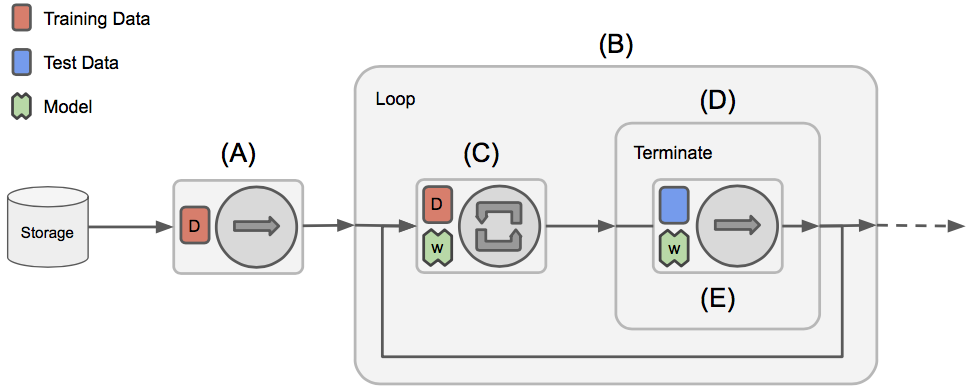
\includegraphics[width=0.9\textwidth]{img/general_pipeline.png}
\caption{Logical plan for iterative-convergent algorithms}
\label{fig:general_pipeline}
\end{figure}
The training process usually starts with loading the input data $D$ from the storage followed by one ore more preprocessing steps (e.g. normalization or standardization as well as splitting the data into training and test set \textbf{(A)}).
A square represents a step of the algorithm, which contains an arbitrary number of input states (e.g. data, model) and some kind of transformation applied to them.
The transformation process is depicted as a circle and can either be applied once (arrow) or multiple times (cyclic arrows) to the state(s) during this particular step.
After applying the preprocessing the actual training process is triggered, which is contained in a loop \textbf{(B)}.
A loop symbolises that the containing steps are executed repeatedly until some termination criterion \textbf{(D)} is statisfied, which is computed in \textbf{(E)}.
For most machine learning algorithms the termination criterion can either be a fixed number of iterations, the change in objective $Q$ between iterations or the generalization performance.
\textbf{(C)} is the actual training step which iteratively refines the model by updates computed from the input data according to \ref{eqn:delta_upd}.
It can already be seen from the example that the framework must be capable of executing a complex sequence of arbitrary control flow operators and transformation steps.



each transformation step must be parallelized as can be seen in Figure \ref{fig:general_pipeline_dist}.
\begin{figure}[ht]
\centering
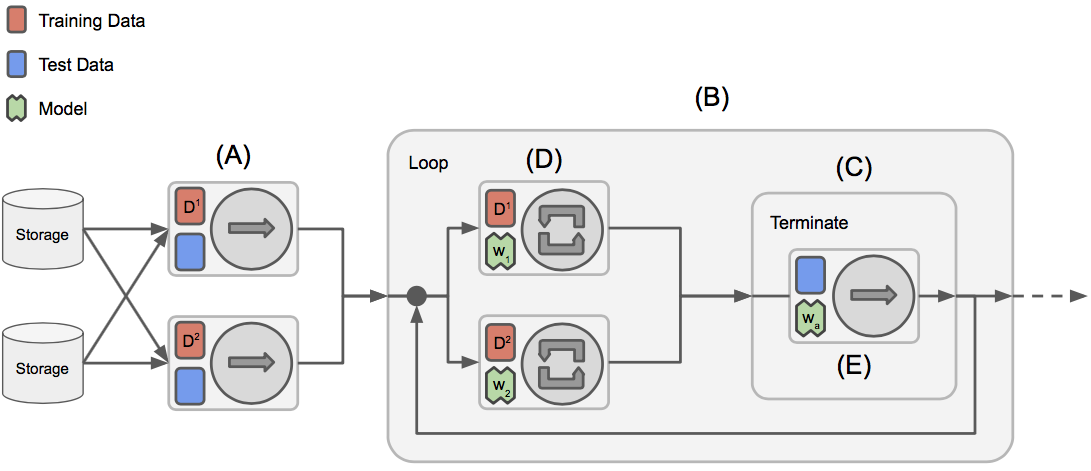
\includegraphics[width=0.9\textwidth]{img/general_pipeline_dist.png}
\caption{Distributed Machine Learning Pipeline for Iterative-convergent Algorithms}
\label{fig:general_pipeline_dist}
\end{figure}
The pipeline described in Figure \ref{fig:general_pipeline} is parallelized with a degree of parallelism of two.
Now each transformation step of the pipeline can be scheduled and executed on two machines in parallel.
It is worth noting that the transformation logic stays the same independently of the degree-of-parallelism, including a dop\footnote{degree of parallelism} of one, which is essentially a single machine.
Only the input and output state(s) of each step have changed in a sense that each parallel step only has access to a part of the orginal state.
Therefore the framework must be able to take a logical plan as in Figure \ref{fig:general_pipeline} and distribute it according to the available resources and possibly additional parameters defined by the developer.
from the description of an algorithm such as elastic-net regularized linear regression.


\textbf{NOTES:} add caption for state, change figure, make termination more generic, it's better to call this control flow
- describe the development flow: developer implements algorithm (specifies states, control flow, applied transformations -> functions), this needs to be identified and mapped into a logical plan by the compiler

\section{Distributed State}
Therefore the actual concern in distributed machine learning is not how to distribute computation but how to distribute the state in order to achieve optimal performance.
As this thesis focuses on machine learning, a state is in general represented by a tensor (e.g. vector or matrix).
The most efficient state distribution depends on properties of the state(s) such as size and sparsity of the input data and model, algorithm used for optimization and infrastructure properties such as available memory and computational resources.

\textbf{NOTES:} add caption for state, change figure, make termination more generic, it's better to call this control flow


\section{Consistency}

NOTES:
- motivate the argumentation with an example machine learning pipeline (elastic-net linear regression) which includes preprocessing (e.g. standard-scaling), iterative model refinement which could be data/model parallel and depending on the size of the model it could either be replicated or partitioned among machines/workers, also a ML pipeline involves generalization error assessment via test/validation dataset, which should be included into the stopping criterion
this should show:
	- what kind of workflow is generaly executed in practice
	- what structure a ml pipeline has and that there are parts that can be run in parallel and in parallel with relaxed constistency/synchronization
	- show what kind of information can be infered from knowledge about the architecture (computational and memory resources, bandwidth, bandwidth quota) and the problem size (size of input data, size of model)
	- what part of distributing a machine learning algorithm can be handled by the system (distributing data, distributing model and computation, scheduling of work) and what needs to be specified by the developer (parallelism, control flow and required states (?), )

- describe the limitations of current state-of-the-art distributed machine learning systems
	- low level primitives
	- not flexible nor expressible api for developing real word machine learning pipelines
	- inference of certain properties depending on hardware architecture (GPU, CPU, FPGA) and algorithm properties
	- distributed control flow
	- focus on optimizing distributed machine learning performance by quick prototyping
	- only concerned with the important parts for going from an exact single machine to a distributed algorithm implementation by specifying data partitioning, topology and constistency management properties (synchronzation requirements/schemes, filter, update/merging strategies)
	- dealing with algorithm related hyperparameters
